\section{Ход работы}

\textit{Ниже написан полнейший БРЕД (точнее компиляция лабораторных), чтобы показать, как делать то или иное действие в латехе. Все совпадения случайны.}

Дана система с произвольной задержкой

$\dot{x} = Ax(t) + A_1 x (t-h), $
$A = 
\begin{bmatrix}
1 &  0\\
4 & 3\\
\end{bmatrix},
A_1 = 
\begin{bmatrix}
-2 & 1 \\
-2 & -6\\
\end{bmatrix}$

$\begin{bmatrix}
\Phi & P - P_2^T (A+A_1)^T P_3 & -h P_2^T A_1\\
* & -P_3 - P_3^T + hR & -h P_3^T A_1\\
* & * & -hR\\
\end{bmatrix} < 0,
$

$\Phi = P_2^T (A+A_1) + (A+A_1)^T P_2, P > 0, R > 0$

Здесь $P_2$ и $P_3$ – произвольные матрицы. В результате решения матричного неравенства выше в MATLAB получена максимальная задержка $h = 0.18$, при которой система является устойчивой. 

Схема моделирования была собрана. Опытным путём удалось установить значение $K_{OC} = 2.5$ - максимальное допустимое, то есть значение при котором система устойчива (это граница устойчивости).

\begin{figure}[H]
    \centering
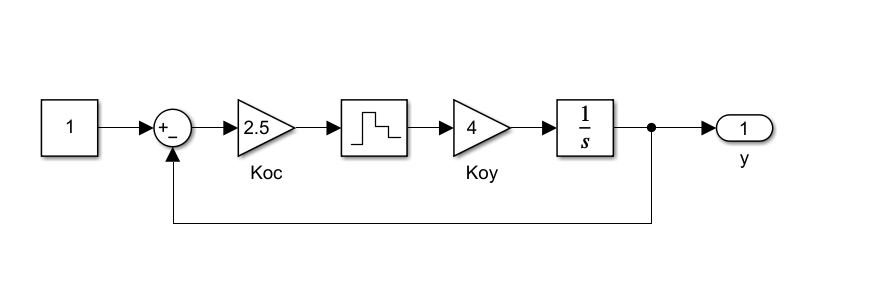
\includegraphics[width=1.\linewidth,center]{assets/images/1.png}
    \caption{Схема моделирования}
    \label{fig:p1}
\end{figure}

% место для вывода про экстраполятор

\subsection{Что-то там про колебательность}

Колебательность процесса при фиксированном периоде квантования $T$ зависит от $K_{OC}$ следующим образом: чем больше $K_{OC}$ - тем больше система будет колебаться, пока не дойдёт до границы устойчивости, на которой она будет вести себя как чисто колебательная система без стремления к нулю.

На графиках ниже можно видеть, как переходный процесс становится всё более колебательным и колебательным. 

Пусть степень устойчивости $\alpha = 0.5$. Тогда

\begin{enumerate}
    \item При $\mu = 3, \; \sigma(A+BK) = \{  -1.3192 \pm 5.2207i,  -0.9915, -1\}$
    \item При $\mu = 1, \; \sigma(A+BK) = \{  -1.1340 \pm 5.5547i,  -0.9361, -1\}$
    \item При $\mu = 0.4, \; \sigma(A+BK) = \{  -0.9402 \pm 5.8582i,  -0.7433, -1\}$
\end{enumerate}


\subsubsection{Графики}

\begin{figure}[H]
    \centering
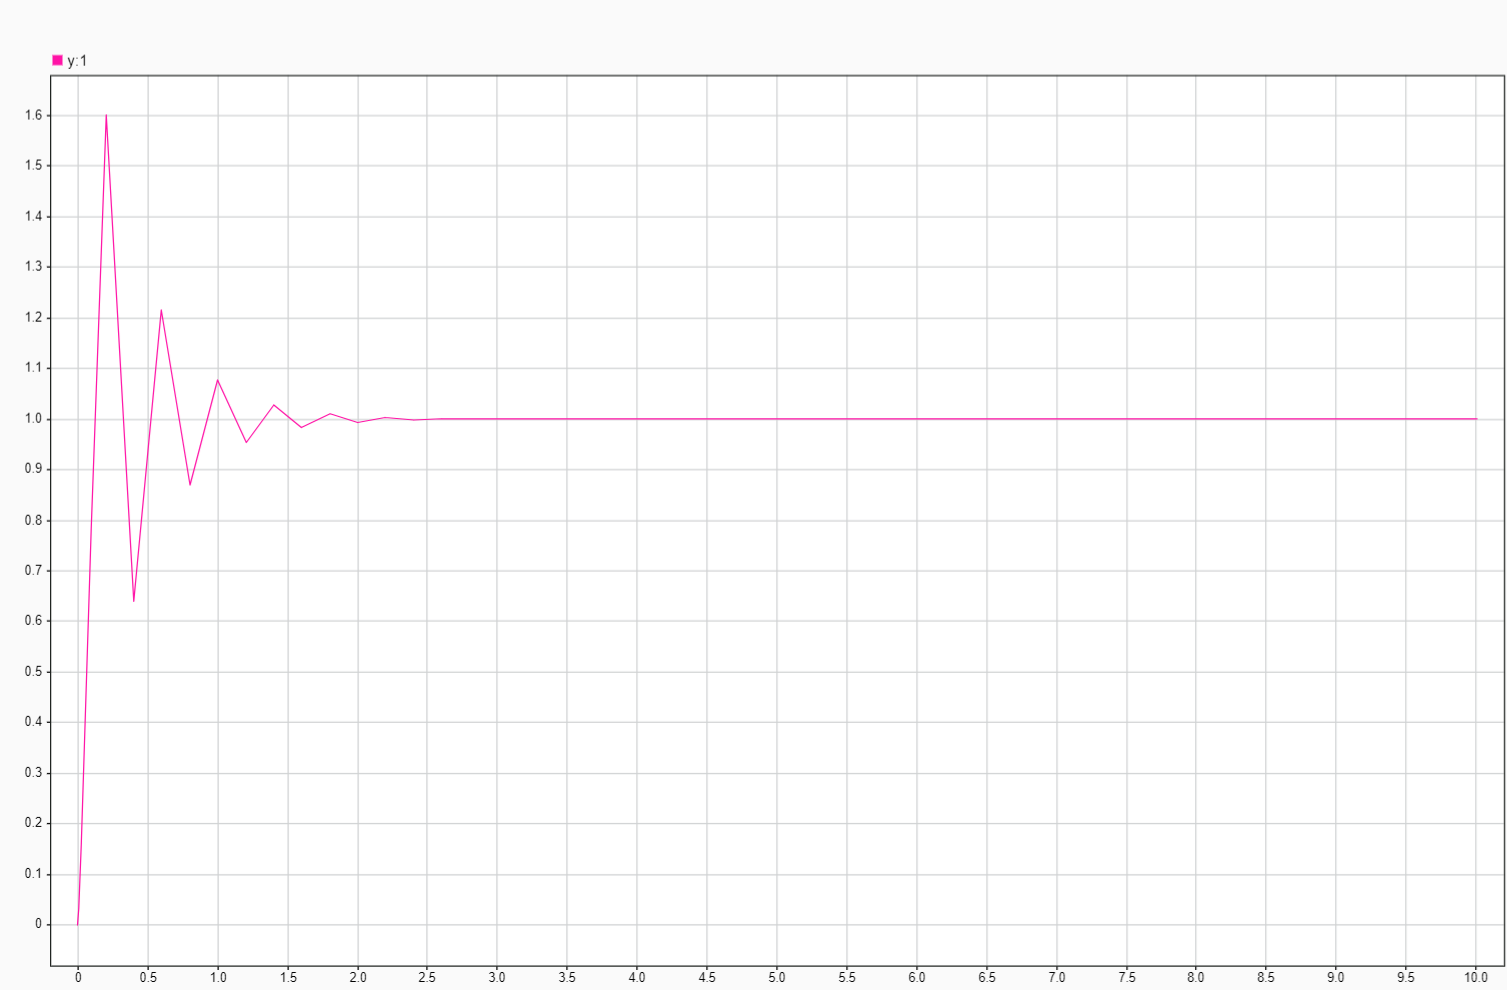
\includegraphics[width=1.\linewidth,center]{assets/images/2.png}
    \caption{График $y(t)$ при $K_{OC} = 2$}
    \label{fig:p2}
\end{figure}


\begin{figure}[H]
    \centering
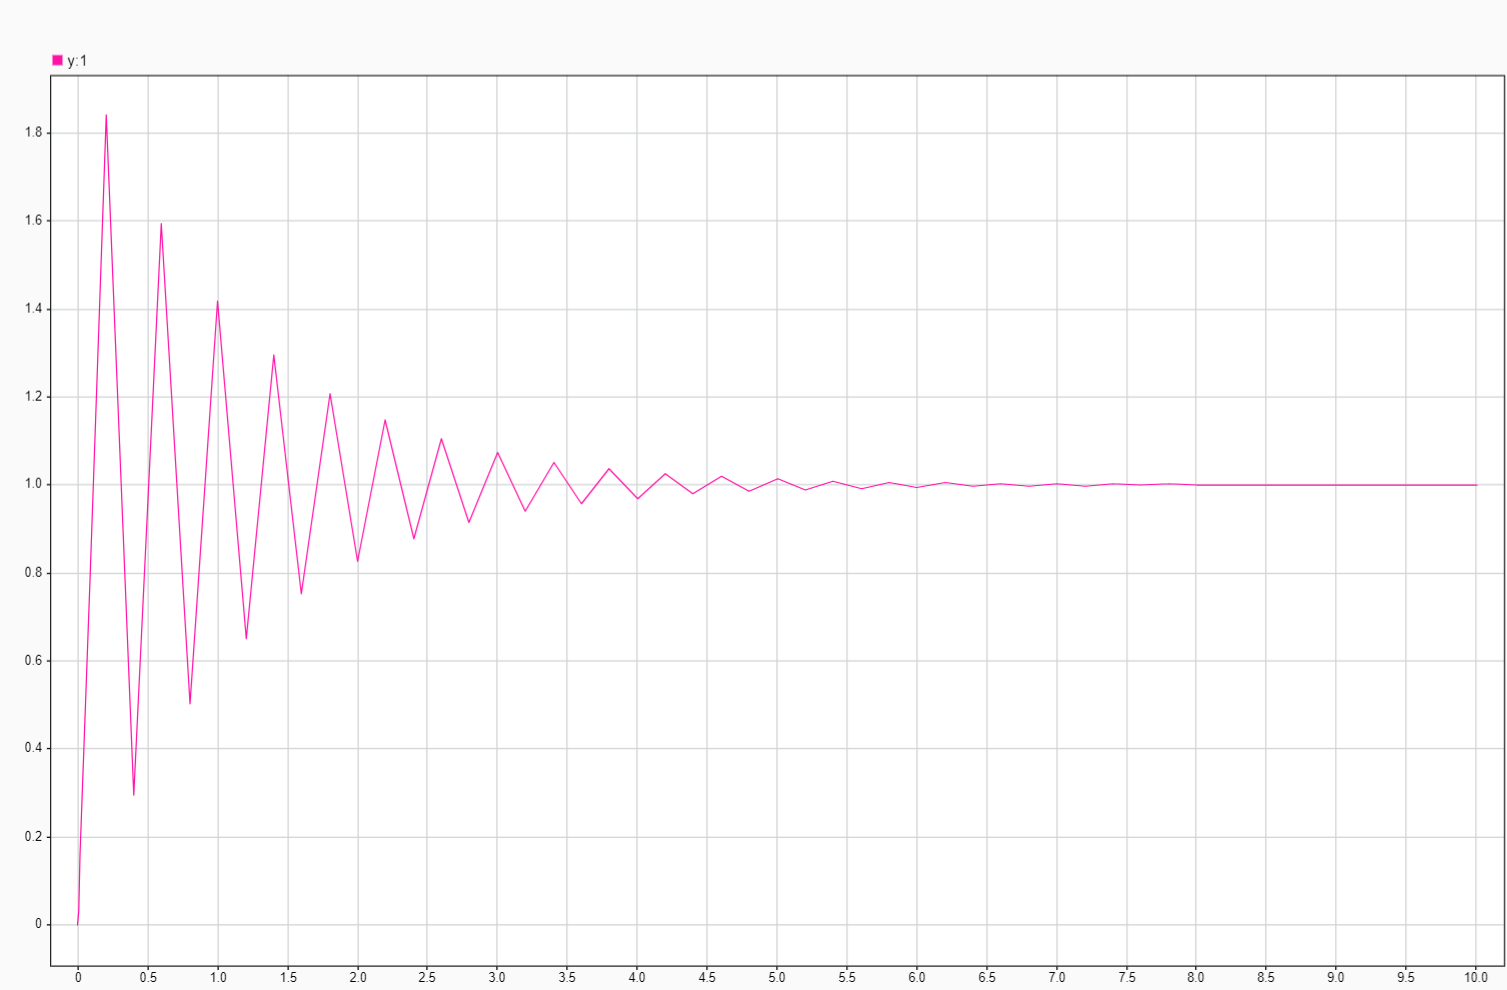
\includegraphics[width=1.\linewidth,center]{assets/images/3.png}
    \caption{График $y(t)$ при $K_{OC} = 2.3$}
    \label{fig:p3}
\end{figure}


\begin{figure}[H]
    \centering
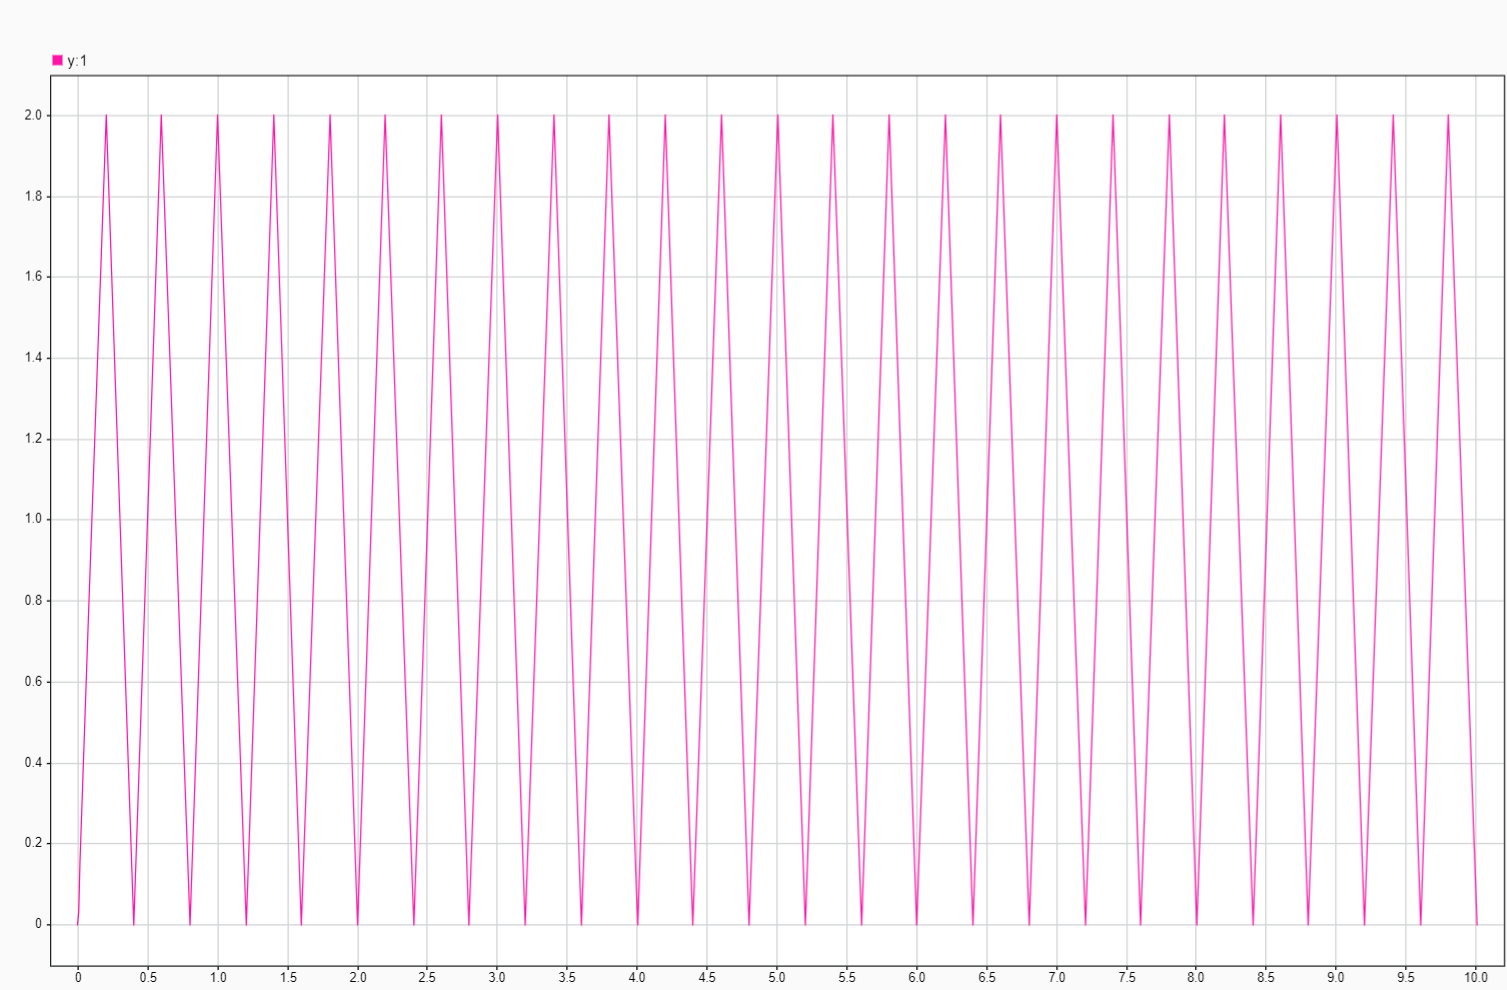
\includegraphics[width=1.\linewidth,center]{assets/images/4.png}
    \caption{График $y(t)$ при $K_{OC} = 2.5$}
    \label{fig:p4}
\end{figure}

\begin{figure}[!htbp]
\centering
\begin{subfigure}{.5\textwidth}
  \centering
  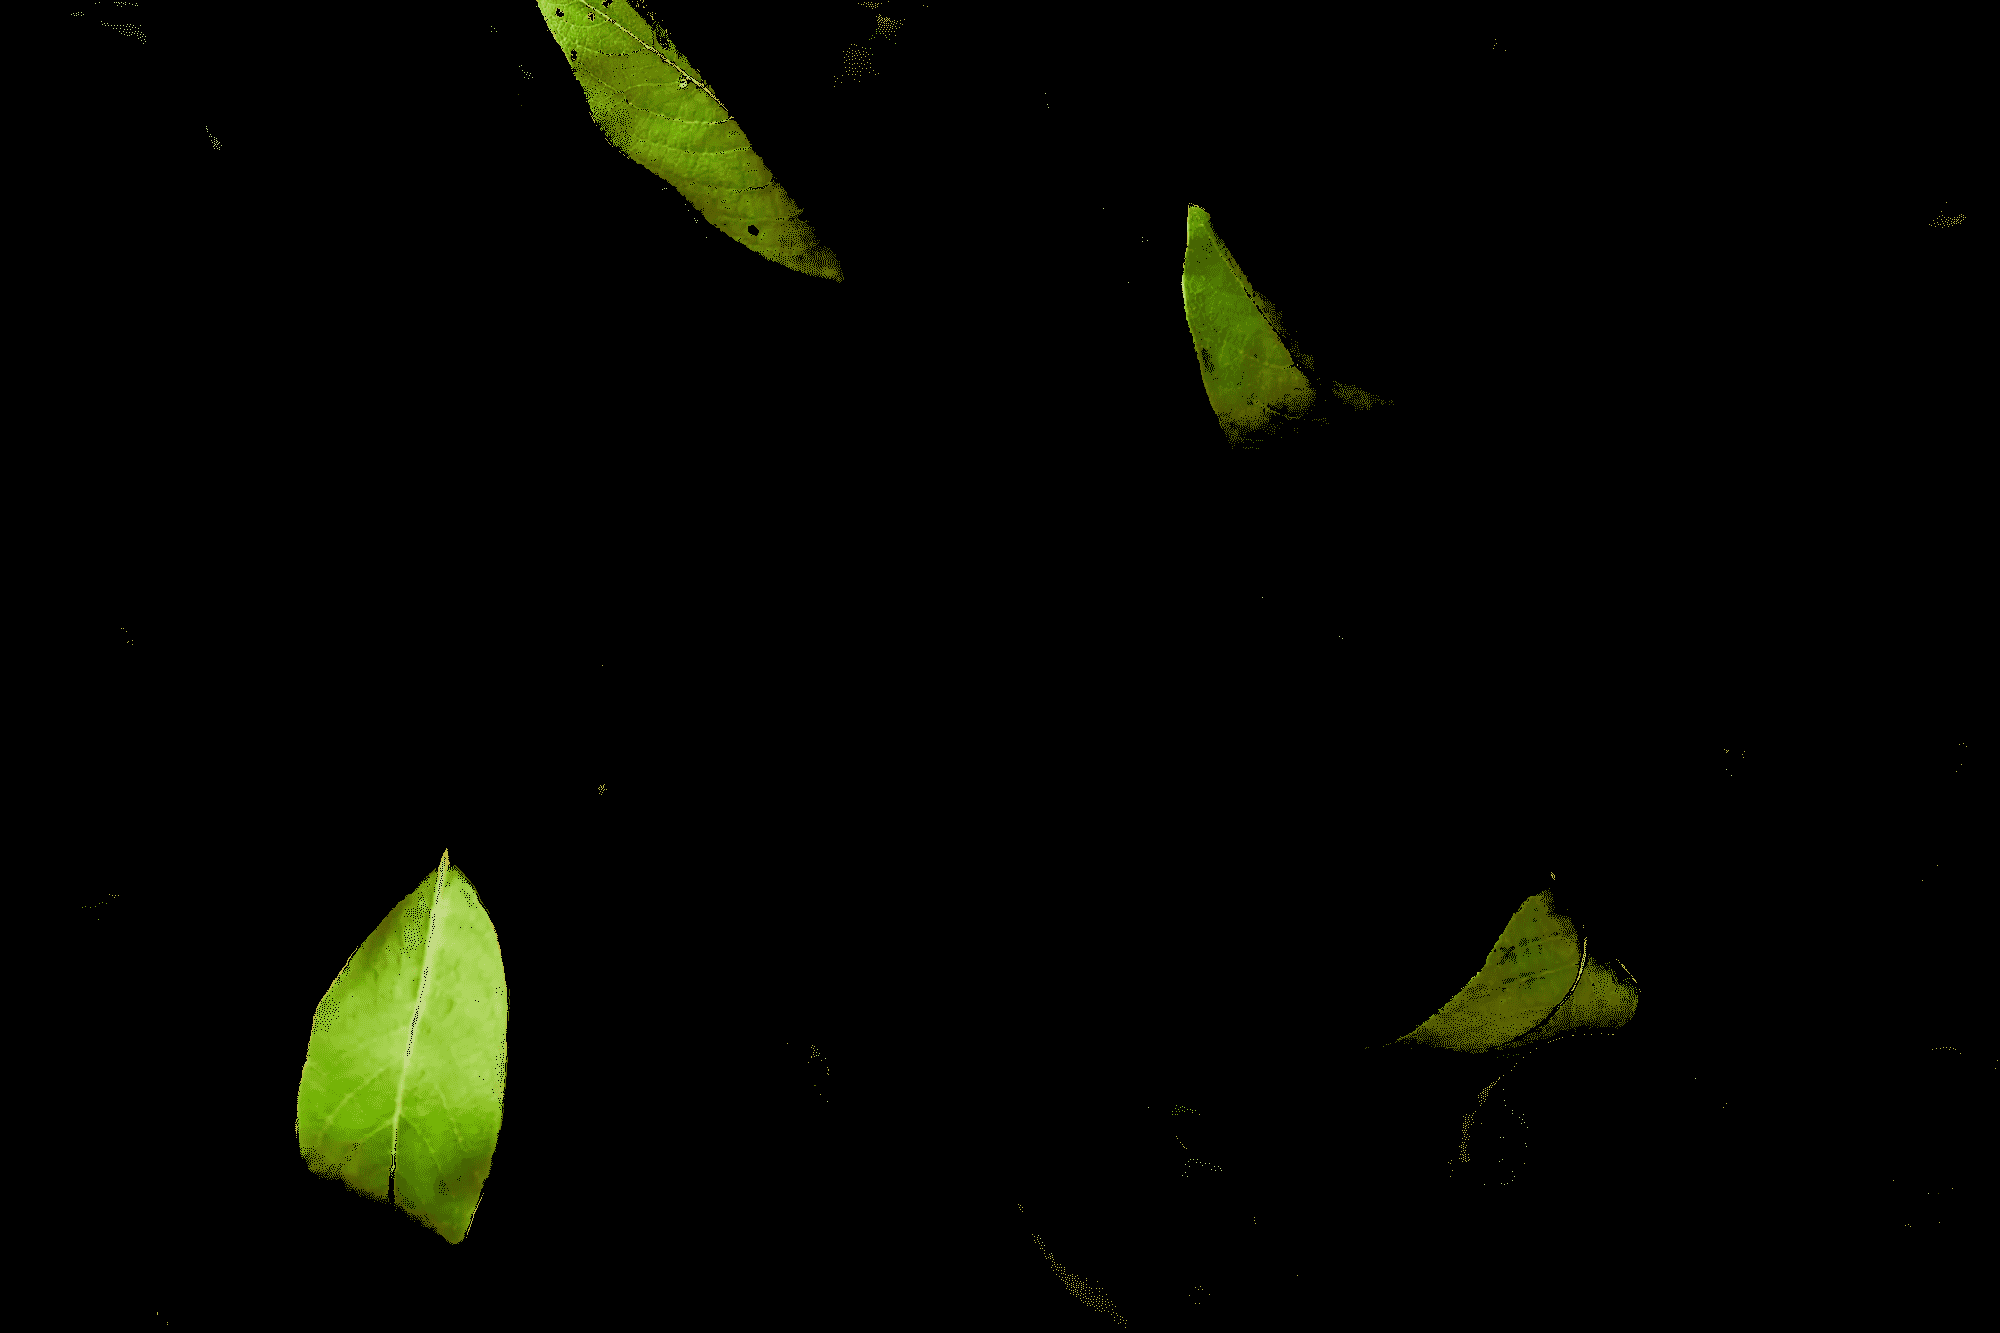
\includegraphics[width=0.8\linewidth]{assets/images/5.png}
  \caption{Зелёные}
  \label{fig:sub1}
\end{subfigure}%
\begin{subfigure}{.5\textwidth}
  \centering
  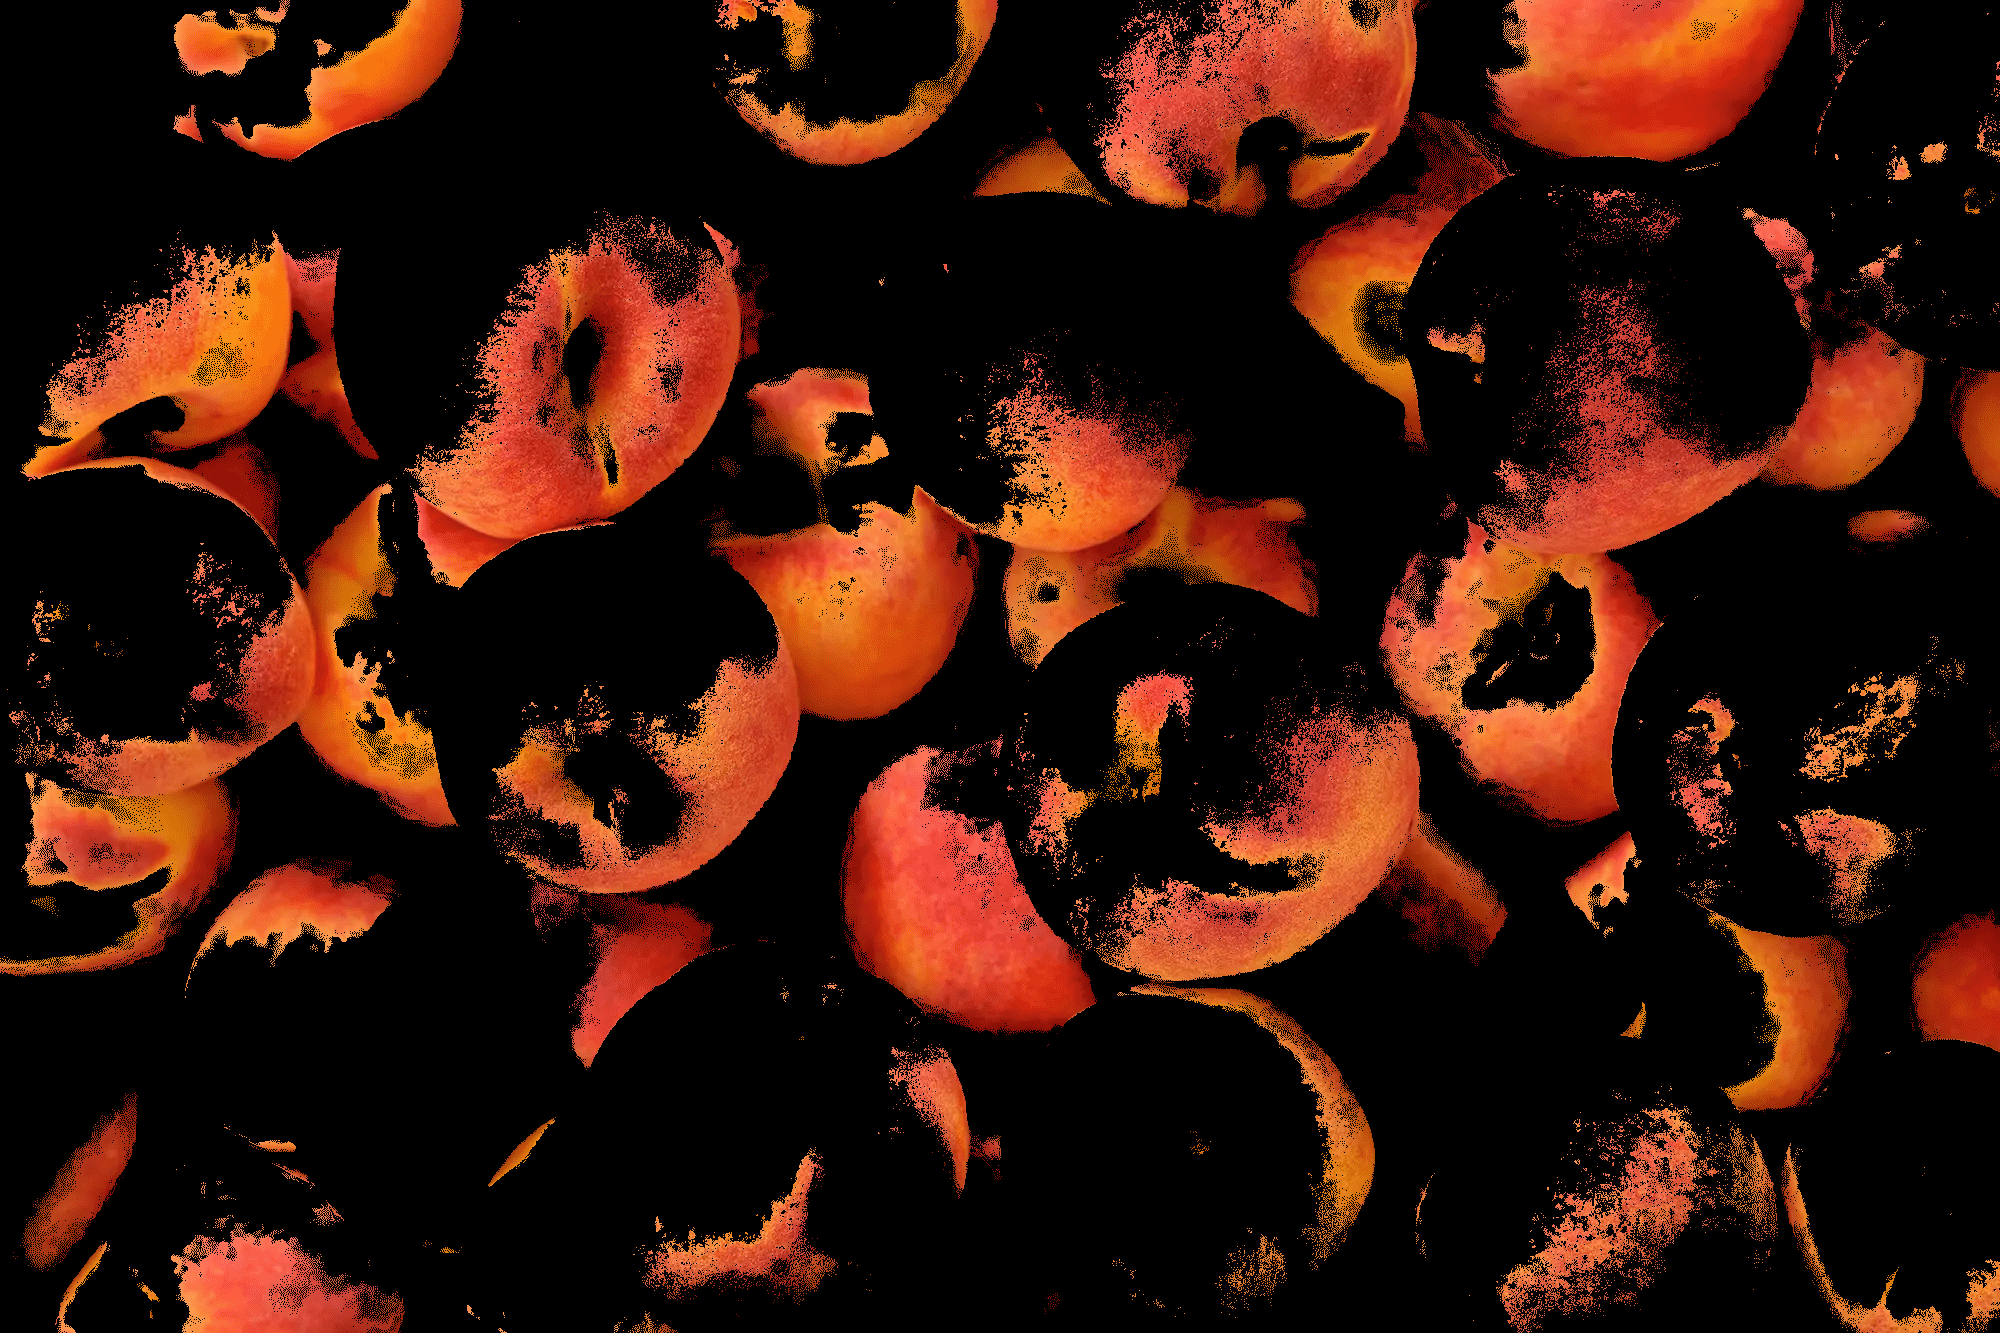
\includegraphics[width=0.8\linewidth]{assets/images/6.png}
  \caption{Оранжевые}
  \label{fig:sub2}
\end{subfigure}
\label{fig:test}
\caption{Сегментированные области}
\end{figure}

Максимальная колебательность наблюдается при $K_{OC} = 2.5$

\subsubsection{Код Python}

\begin{lstlisting}[language=Python, caption=Импорт и обычная бинаризация]
import cv2
from google.colab.patches import cv2_imshow
from matplotlib import pyplot as plt
import numpy as np
from math import *
import skimage
from skimage import data, io, filters

I=cv2.imread("pic.jpg",cv2.IMREAD_GRAYSCALE)
cv2_imshow(I)
t=127
ret,Inew=cv2.threshold(I,t,255,cv2.THRESH_BINARY)
plt.imshow(Inew)
\end{lstlisting}

Ссылка на первый рисунок: \ref{fig:p1}